\section{Theoretical Framework}
\label{sec:theory}
In this section we introduce the theoretical guarantees of our algorithm and prove them. Note that the total error in the frequency estimation of a true HH flow might originate from several parts of the algorithm. The first error type, is the \textit{\ee} due to the usage of shared estimators in the \sea. This relative error is bounded by $\delta$ as guaranteed from the original CEDAR scheme.

The second error type, is the one introduced to the estimation of HH flows for not propagating early enough from the \sfa\ to the \cs. We denote it by \textit{\pe} and show that the probability of a HH flow not to propagate to the \cs\ is small and it decreases with the increase of the size of the \sfa. The third type of error is the error introduced to the estimation of HH flows due to the eviction of such flows from the \cs. We denote it by \textit{\eve}, and as before we show that the probability of a HH flow to be evicted either by a HH or a non HH flow is small and decreases with the increase of the size of the \cs.

\begin{maybeappendix}{theory}
We introduce two less famous variants of Chernoff bounds that bound the probability of choosing elements from subsets when considering a random sample of the universe of a given set. These variants are relevant to the networking domain, since one can consider a trace as the universe set and its subsets are the packets of each active flow.

Lemma~\ref{lemma:lower_tail} bounds the probability of having ``too many" elements of a given flow in a sampled subset of the trace. In the networking domain, the set $A$ is the trace and the subset $B$ contains the packets of a given flow. This Lemma conjectures on the number of packets of a given flow within a sample $S$ of size $k$, the bound is parameterized with $\delta$ that represents the deviation from the mean $\frac{k|B|}{|A|}$ ($k$ packets each with probability of $\frac{|B|}{|A|}$ to be in $B$). Lemma~\ref{lemma:upper_tail} follows the same logic of Lemma~\ref{lemma:lower_tail} regarding the probability of having ``too few" elements of a given flow in the sampled subset.

\begin{lemma}[Extended Chernoff Lower Tail Bound]
\label{lemma:lower_tail}
Consider a set $A$ and its subset $B$. Suppose we pick an integer $0<k<|A|$ and a random subset $S$ of size $k$, then for $0<\delta \leq 1$ we have:

$Pr\left[|S \cap B| \leq \frac{(1-\delta)|B|k}{|A|}\right] \leq e^{-\frac{|B|k\delta^2}{2|A|}}$
\end{lemma}
\begin{proof}
can be found in~\cite{bounds}.
\end{proof}

\begin{lemma}[Extended Chernoff Upper Tail Bound]
\label{lemma:upper_tail}
Consider a set $A$ and its subset $B$. Suppose we pick an integer $0<k<|A|$ and a random subset $S$ of size $k$, then for $0<\delta$ we have:

$Pr\left[|S \cap B| \geq \frac{(1+\delta)|B|k}{|A|}\right] \leq e^{\frac{-|B|k\delta^2}{(2+\delta)|A|}}$
\end{lemma}
\begin{proof}
can be found in~\cite{bounds2}.
\end{proof}

\end{maybeappendix}

We denote by $F_{h_1(f)}$ the set of flows that are mapped to the same entry by $h_1$ as $f$, i.e., $F_{h_1(f)} = \{g\in F | h_1(g)=h_1(f)\}$, and by $\gamma_f$ the portion of flow $f$ from the whole trace, i.e., $\gamma_f N$ is the number of packets of flow $f$. Furthermore, we denote by $\Gamma_f$ the sum of portions of flows mapped to the same entry as $f$ by $h_1$, i.e., $\Gamma_f=\sum_{g\in F_{h_1(f)}} \gamma_g$. We use $HH$ to denote the set of HH flows and the sum of their portions by $\Gamma_{HH}=\sum_{f \in HH}\gamma_f$.

Theorem~\ref{thm:found} proves that any HH will be propagated to the \cs\ with high probability by showing that the probability of not propagating is
$(\frac{1-\Gamma_{HH}}{k})^{\gamma_f N v_0-1}$ and that this probability decreases when $k$ increases, i.e., more memory allocated to the \sfa.

\begin{theorem}
\label{thm:found}
Given a HH flow $f$ and a \sfa\ of size $k$, if we assume uniformity in the appearances of $F_{h_1(f)}$, then the probability of $f$ not propagating to the \cs\ is $(\frac{1-\Gamma_{HH}}{k})^{\gamma_f N v_0-1}$.
\end{theorem}

\begin{proof}
We first note that for a HH flow $f$, the term $\Gamma_f-\gamma_f$ represents the sum of portions of all other flows besides $f$ that are hashed to $h_1(f)$. Since $h_1$ is a uniform hash function then $\Gamma_f-\gamma_f = \frac{1-\Gamma_{HH}}{k}$.

The probability of HH flow $f$ not to propagate to the \cs, is the the product of the probabilities of it being evicted between its $i^{th}$ and $i+1^{th}$ sampled packets, $\forall i\geq 2$. Since $f$'s portion is $\gamma_f$, and assuming uniformity of appearances of $F_{h_1(f)}$, then the probability of it being evicted between its $i^{th}$ and $i+1^{th}$ sampled packet is $\frac{(\Gamma_f-\gamma_f) v_0 N / (\gamma_f + 1)}{v_0 N / (\gamma_f + 1)} = \Gamma_f-\gamma_f$.

Thus, the probability of $f$ not propagating is $\prod^{\gamma_f N v_0}_{i=2} (\Gamma_f - \gamma_f) = (\frac{1-\Gamma_{HH}}{k})^{\gamma_f N v_0 -1}$.
\end{proof}

\ignore{
We start by introducing Lemma~\ref{lem:sum_to_prod} that bounds the maximal product of positive integer variables given their sum as a constraint.  This is a straightforward conclusion from the fact that geometric mean of a non-empty data set of positive numbers is always at most their arithmetic mean.

\begin{lemma}
\label{lem:sum_to_prod}
Assume $x_1,...,x_n$ are positive integers and that $\sum_{i=1}^{n}x_i=s$, then $\prod_{i=1}^{n}x_i \leq (\frac{s}{n})^n$.
\end{lemma}
\dannysays{Note that I changed the Lemma (no +1) and replaced the proof by a sentence before the Lemma}

\begin{proof}

To achieve this bound, we first solve the straightforward maximization problem and then bound the maximal product of the solution.
Let us assume in contradiction that in the solution there are indices $i,j$ that $x_i>x_j+1$, then $(x_i-1)(x_j+1)>x_ix_j$ thus we can replace $x_i$ by $x_i-1$ and $x_j$ by $x_j+1$ and acquire a greater product, thus, $|x_i-x_j|\leq1$ for all $i,j$.
%
Examining the solution under this constraint yields that only two integer values can appear, denoted by $a, a+1$, and they appear $n-k, k$ times respectively. Then $s=(n-k)a+k(a+1)$ which yields that $k=s \bmod n$ and $a=\lfloor \frac{s}{n} \rfloor$.

Then the maximal product is
$\lfloor\frac{s}{n}\rfloor^{n-(s \bmod n)} * \lfloor \frac{s}{n} + 1 \rfloor^{s \bmod n}$
which is at most $(\frac{s}{n}+1)^{n}$.
\end{proof}

\begin{theorem}
\label{thm:foun1}
If flow $f$ is a heavy hitter flow, then the probability of $f$ not propagating to the \cs\ is $o(1)$.
\end{theorem}
\begin{proof}
Let us examine the appearances of packets of flow $f$, and denote by $S_i$ the packets between appearances of packets $i-1$ and $i$ of $f$. We note that $f$ will not propagate to the the \cs\ if and only if in any $S_i$ there is at least one packet from $F_{h1(f)}/f$. The probability of such event is $(\Gamma_f-\gamma_f)|S_i| < \Gamma_f|S_i|$. Thus the probability of $f$ not propagating is bounded by $\prod_{i=1}^{\gamma_f N/v_0} \Gamma_f|S_i|=\Gamma_f\prod_{i=1}^{\gamma_f N/v_0}|S_i|$.

We use Lemma~\ref{lem:sum_to_prod} to bound this probability, by noting that $s=\sum_{|S_i|}=\frac{\Gamma_F N}{v_0}$ since this is the number of packets that gets sampled and mapped to $h1(f)$, also $n=\frac{\gamma_f N}{v_0}$, thus $\frac{s}{n}=\frac{\Gamma_f}{\gamma_f}$ and the product is bounded by $(\frac{\Gamma_f}{\gamma_f} + 1)^{\gamma_f N /v_0}$ and the probability by $\Gamma_f(\frac{\Gamma_f}{\gamma_f} + 1)^{\gamma_f N /v_0}$. We recall that $\gamma_f, \Gamma_F, \phi$ are constants and that $v_0=v \phi N$  where $v$ is the propagation parameter, then the probability is of the form $c_1*c_2^{c_3/v}$ where $c_3=\frac{\gamma_f}{\phi}>1$ and we can have it as small as we wish by setting $v$ accordingly.
\end{proof}

}

The algorithm will give a frequency estimation within the relative error of the true frequency for any flow in the \cs, however, this estimation holds from the moment the flow was propagated to the \cs\ and this does not happen on the first packet of the flow. Thus, the overall error of the algorithm consists of the guaranteed estimation error by the \sea\ mechanism, and the error introduced by the propagation mechanism in the \sfa. Theorem~\ref{thm:found} shows that we can control the probability of a HH not propagating to the \cs\ to be as small as we wish.\ignore{, indicating that the \pe\ is constant.}

If we assume uniformity in the appearances of $F_{h_1(f)}$, then Theorem~\ref{thm:uni} shows we can bound the expected \pe\ by $v_0\left(\frac{1}{(1-1/k)^{1/ \gamma_f+1}}-1\right)$, where $k$ is the size of the \sfa. It is worthy to note that the bigger $k$ the smaller the expected \pe.

\begin{theorem}
\label{thm:uni}
Given a HH flow $f$, if we assume uniformity in the appearances of $F_{h_1(f)}$, then the expected \pe\ of flow $f$ is constant and at most $v_0\left(\frac{1}{(1-1/k)^{1/ \gamma_f+1}}-1\right)$.
\end{theorem}
\begin{proof}
We start by noting that since $h_1$ is a hash function and that the size of the \sfa\ is $k$ then $\Gamma_f = \frac{1}{k}$, this means that all packets are hashed into $k$ buckets and the portion of the flows hashed into the same bucket as $f$ is $\frac{1}{k}$.

If we consider two packets of flow $f$, then in between them there are at most $\frac{2v_0}{\gamma_f+1}$ other packets. For $f$ to propagate, none of these packets which gets sampled should be from $F_{h_1(f)}$ and this happens with probability $p_s=(1-\Gamma_f)^{\frac{2v_0}{2v_0(\gamma_f+1)}}\leq(1-\frac{1}{k})^{\frac{1}{\gamma_f}+1}$.

Since the \pe\ affects $f$'s total error until $f$ gets propagated, then the event is geometrically distributed with probability of success $p_s$ and have an expectation of $\frac{1}{p_s}$. Since the flow is propagated with estimation $v_0$ then the expected \pe\ is $v_0\left(\frac{1}{(1-1/k)^{1/ \gamma_f+1}}-1\right)$.
\end{proof}


\begin{maybeappendix}{theory}
In Lemma~\ref{lemma:not_prop} we prove that the error introduced by the propagation mechanism is at most $\frac{1}{1-e^{\frac{-\frac{1}{m}(1-2m)^2}{2}}}$, where $m=\frac{\phi}{\gamma c}$.

\begin{lemma}
\label{lemma:not_prop}
Given a flow $f$ of frequency $\gamma N$ ($0\leq \gamma \leq 1)$, then the probability of not propagating to the \cs\ from a \sfa\ of size $\frac{c}{\phi}$, is at most ${1-e^{\frac{-\frac{1}{m}(1-2m)^2}{2}}}$, where $m=\frac{\phi}{\gamma c}$.
\end{lemma}

\begin{proof}
Follows from Lemma~\ref{lemma:lower_tail} with $\frac{(1-\delta)|B|k}{|A|}=2$, since a flow will not propagate to the \cs\ if and only if there are no 2 occurrences in $\frac{c}{\phi}$ packets which is the size of \sfa.
\end{proof}

\begin{lemma}
\label{lemma:not_prop_geo}
Given a true heavy hitter flow $f$ of frequency $\gamma N$ ($\phi \leq \gamma \leq 1)$, then the expected addition to the estimation error due to the \sfa\ propagation mechanism is $\frac{1}{1-e^{\frac{-\frac{1}{m}(1-2m)^2}{2}}}$.
\end{lemma}

\begin{proof}
As estimation error due to the array propagation mechanism is added, only when a true heavy hitter flow is encountered at most once during $\frac{c}{\phi}$ packets and not propagated to the \cs. Thus the expectancy of the error is distributed geometrically with probability of success of ${1-e^{\frac{-\frac{1}{m}(1-2m)^2}{2}}}$.
\end{proof}

Figure~\ref{fig:prop_err} depicts the \pe\ behaviour for values of $0 \leq \frac{\phi}{\gamma} \leq 3$. The interesting values are when $\gamma \geq \phi$, since the analysis of the \pe\ is only relevant for true heavy hitter flows. It is evident that for the most of the domain, the \pe\ is negligible, but yet it is unbounded around $0.5$ for $c=1$. Which means we can not guarantee a constant negligible \pe\ for true heavy hitters that are about twice the threshold. For that, we facilitate the parameter $c$, the constant multiplier in the size of \sfa, to push the unbounded domain outside of $[0,1]$ domain.

It is worthy to note that it is not enough to use $\frac{2}{phi} (c=2)$ entries in \sfa, since the unbounded domain will reside around $1$ which mean we will have a greater \pe\ for flows around the threshold and usually these are the flows that are the hardest to reason about due to the sensitivity in classifying them. While using $c\geq 4$ will increase the size of \sfa, however this increase is still constant with great benefit since it will push the unbounded domain around $2$, which contains only non heavy hitter flows.

\begin{figure}
    \centering
    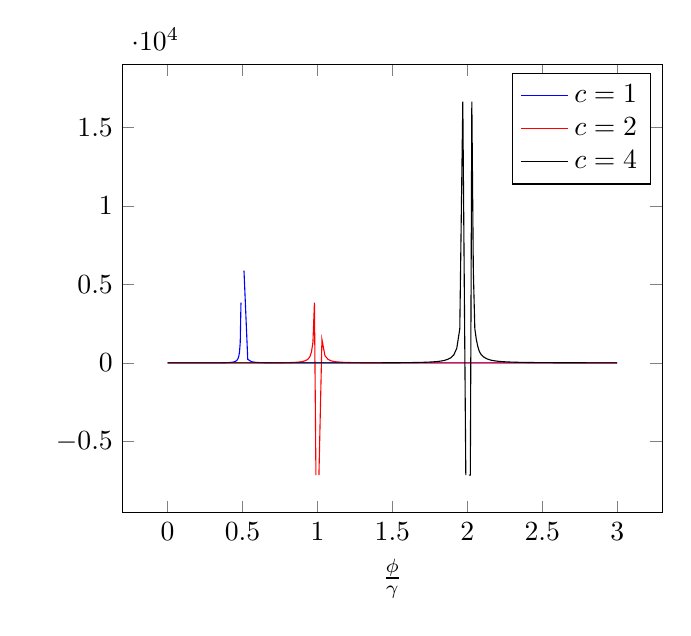
\begin{tikzpicture}
        \begin{axis}[ 
            xlabel=$\frac{\phi}{\gamma}$,
            ylabel={\pe}
        ] 
        \addplot [samples=100, domain=0:0.49, color=blue]{1/(1-e^((-1/(x)*(1-2*x)^2)/(2)))}; 
        \addplot [forget plot, samples=100, domain=0.51:3, color=blue]{1/(1-e^((-1/(x)*(1-2*x)^2)/(2)))}; 
        \addplot [samples=100, domain=0:0.99, color=red]{1/(1-e^((-1/(1/2*x)*(1-x)^2)/(2)))}; 
        \addplot [forget plot,samples=100, domain=1.01:3, color=red]{1/(1-e^((-1/(1/2*x)*(1-x)^2)/(2)))};
        \addplot [samples=100, domain=0:1.99, color=black]{1/(1-e^((-1/(1/4*x)*(1-1/2*x)^2)/(2)))}; 
        \addplot [forget plot,samples=100, domain=2.01:3, color=black]{1/(1-e^((-1/(1/4*x)*(1-1/2*x)^2)/(2)))};
        \addlegendentry{$c=1$}
        \addlegendentry{$c=2$}
        \addlegendentry{$c=4$}
    \end{axis}
    \end{tikzpicture}
    \caption{The \pe\ as function of $\frac{\phi}{\gamma}$}
    \label{fig:prop_err}
\end{figure}
\end{maybeappendix}

In order to analyse the \eve\ we will have to reason about the probability of HH flows to evict each other from the \cs\ and about the probability of non HH flows to evict HH flows from the \cs.

It is trivial to see that the probability of a HH flow to evict another HH flow from the \cs\ is controlled by the size of the \cs, $M$. Since there are at most $\frac{1}{\phi}$ heavy hitter flows, the probability of being evict by another HH is at most $\frac{\frac{1}{\phi}-1}{M}$ and it is enough to choose $\frac{1}{\phi} << M$ to get this probability as small as we wish.

\ignore{
\begin{lemma}
\label{lemma:nonhhhevic1}
Given a HH flow in the \cs\ with estimation $v_i$, the probability of being evicted by a non HH flow is $o(1)$.
\end{lemma}
\begin{proof}
In order for a non HH to evict a HH, it should go through the following steps: (1) enter the \sfa, (2) get propagated to the \cs\ and (3) evict the HH flow. The probability of the first step is $\frac{1}{v_0}$, the probability of the second step is at most $\frac{1}{v_0}$ (since it could get evicted itself from the \sfa) and the probability of the last step is $\frac{v_0}{v_i}$. Thus, the probability of evicting the HH flow is at most $\frac{1}{v_0v_i}$ which can be small as we wish by controlling $v$ since $v_0=v\phi N$.
\end{proof}
}
\begin{theorem}
\label{lemma:nonhhhevict}
Given a \cs\ of size $M$, and a HH flow $f$ with estimation $v_i$, the probability of $f$ being evicted by a non HH flow $g$ is at most $1/(M v N \phi \gamma_g^2 v_i)$.
\end{theorem}
\begin{proof}
In order for a non HH flow to evict a HH flow, it should go through the following steps: (1) enter the \sfa, (2) get propagated to the \cs\, (3) collide with $f$ when being hashed with $h_2$, and (4) evict $f$. The probability of the first step is at most $\frac{1}{v_0 \gamma_g}$, the probability of the second step is at most $\frac{1}{v_0 \gamma_g}$ (since it could get evicted itself from the \sfa), the probability of the third step is $\frac{1}{M}$ and the probability of the last step is $\frac{v_0}{v_i}$. Thus, the probability of evicting the HH flow $f$ by non HH flow $g$ is at most $\frac{1}{M v N \phi \gamma_g^2 v_i}$ which approaches $0$ as $M$ grows and can be small as we wish by controlling $v$.
\end{proof}

From the observation about the small as we wish probability of HH flows evicting each other and from Theorem~\ref{lemma:nonhhhevict}, we conclude that \eve\ is constant. Later our evaluation shows that after certain size of the \cs, there is no more effect on the algorithm's Detection Rate and False Positive Rate, supporting the claim that by increasing $M$ one can lower the \eve.

\begin{maybeappendix}{theory}

propagate to the \cs. Lemma~\ref{lemma:prop} reasons about the probability of propagating a given flow to the \cs\ given its size.

\begin{lemma}
\label{lemma:prop}
Given a flow $f$ of frequency $\gamma N$ ($0\leq \gamma \leq 1)$, then the probability of propagating to the \cs\  from the \sfa\ of size $\frac{c}{\phi}$, is at most $e^{\frac{-\frac{1}{m}(1-2m)^2}{3-2m}}$, where $m=\frac{\phi}{\gamma c}$.
\end{lemma}
\begin{proof}
Follows from Lemma~\ref{lemma:upper_tail} with $\frac{(1+\delta)|B|k}{|A|}=2$, since a flow will propagate to the \cs\ if and only if there are at least 2 occurrences in $\frac{c}{\phi}$ packets which is the size of \sfa.
\end{proof}

Lemma~\ref{lemma:avg_prop} conjectures on the probability of propagating the average non heavy hitter flow. Let us assume $F$ active flows in the trace where $H$ of them are true heavy hitters (we note that $H\leq\frac{1}{\phi})$, and that the portion of the true heavy hitters flows is $\phi_H$. Since usually that are much more active flows that heavy hitter flows ($H<<F$) \ignore{and the portion of heavy hitter flow is much bigger than those of non heavy hitters flows ($(1-\phi_H) << 1$)}, it makes sense to assume uniformity in the distribution of sizes of the non heavy hitter flows. Thus, the average frequency of a non heavy hitter flow is $\Bar{\gamma} = \frac{1-\phi_H}{F-H}$.

\begin{lemma}
\label{lemma:avg_prop}
The probability of propagating a non heavy hitter flow from a trace with $F$ active flows and $H$ heavy hitter flows of total portion $\phi_H$, is at most
$e^{\frac{-\frac{1}{\bar{m}}(1-2\bar{m})^2}{3-2\bar{m}}}$ where $\bar{m}=\frac{\phi}{c\bar{\gamma}}$.
\end{lemma}
\begin{proof}
Follows from Lemma~\ref{lemma:prop} and the above explanation.
\end{proof}

In Lemma~\ref{lemma:eve} we propose an upper bound on the probability of evicting a true heavy hitter flow from the \cs. While this probability is not bounded, it can be reduced by increasing $M$ and we will show later in the evaluation section that eviction does not happen of any practical settings. 

\begin{lemma}
\label{lemma:eve}
Given a \cs\ of size $M$ and a true heavy hitter flow $f$ and let us denote by $p$ the probability of an average non heavy hitter flow to propagate to the \cs\ presented in Lemma~\ref{lemma:avg_prop}, then the probability of $f$ to be evicted from the candidate set is at most $p^{M-(\frac{1}{\phi}-1)}$.
\end{lemma}
\begin{proof}
A true heavy hitter flow will be evicted from \cs\ if and only if the \cs\ becomes full. Since $M > \frac{1}{\phi} \geq H$, it will be evicted if enough non heavy hitter flows will be propagated, i.e. if $M-(H-1)$ non heavy hitter flows was propagated. This will happen with probability $p^{M-(H-1)}$.
\end{proof}

\ignore{
\begin{figure}
    \centering
    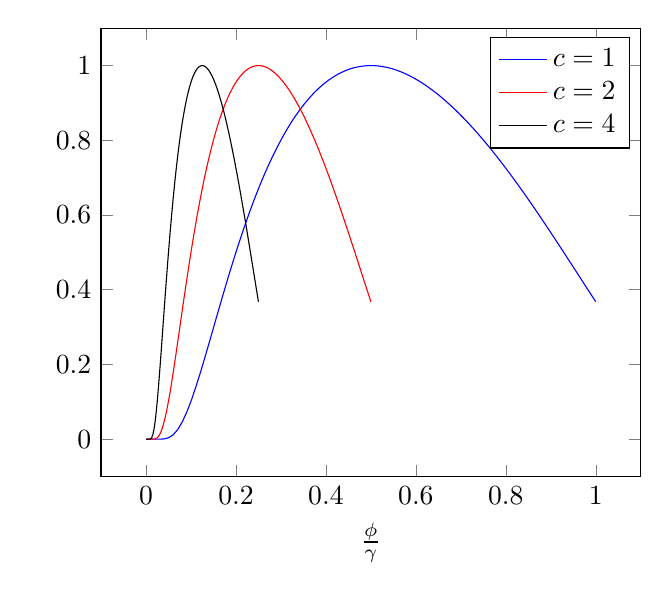
\begin{tikzpicture}
        \begin{axis}[ 
            xlabel=$\frac{\phi}{\gamma}$,
            ylabel={\pe}
        ] 
        \addplot [samples=100, domain=0:1, color=blue]{e^((-1/(x)*(1-2*x)^2)/(3-2*x))}; 
        \addplot [samples=100, domain=0:0.5, color=red]{e^((-1/(2*x)*(1-4*x)^2)/(3-4*x))}; 
        \addplot [samples=100, domain=0:0.25, color=black]{e^((-1/(4*x)*(1-8*x)^2)/(3-8*x))}; 
        \addlegendentry{$c=1$};
        \addlegendentry{$c=2$};
        \addlegendentry{$c=4$};
    \end{axis}
    \end{tikzpicture}
    \caption{The \pe\ as function of $\frac{\phi}{\gamma}$}
    \label{fig:eve}
\end{figure}
}
\end{maybeappendix}